\documentclass[1p]{elsarticle_modified}
%\bibliographystyle{elsarticle-num}

%\usepackage[colorlinks]{hyperref}
%\usepackage{abbrmath_seonhwa} %\Abb, \Ascr, \Acal ,\Abf, \Afrak
\usepackage{amsfonts}
\usepackage{amssymb}
\usepackage{amsmath}
\usepackage{amsthm}
\usepackage{scalefnt}
\usepackage{amsbsy}
\usepackage{kotex}
\usepackage{caption}
\usepackage{subfig}
\usepackage{color}
\usepackage{graphicx}
\usepackage{xcolor} %% white, black, red, green, blue, cyan, magenta, yellow
\usepackage{float}
\usepackage{setspace}
\usepackage{hyperref}

\usepackage{tikz}
\usetikzlibrary{arrows}

\usepackage{multirow}
\usepackage{array} % fixed length table
\usepackage{hhline}

%%%%%%%%%%%%%%%%%%%%%
\makeatletter
\renewcommand*\env@matrix[1][\arraystretch]{%
	\edef\arraystretch{#1}%
	\hskip -\arraycolsep
	\let\@ifnextchar\new@ifnextchar
	\array{*\c@MaxMatrixCols c}}
\makeatother %https://tex.stackexchange.com/questions/14071/how-can-i-increase-the-line-spacing-in-a-matrix
%%%%%%%%%%%%%%%

\usepackage[normalem]{ulem}

\newcommand{\msout}[1]{\ifmmode\text{\sout{\ensuremath{#1}}}\else\sout{#1}\fi}
%SOURCE: \msout is \stkout macro in https://tex.stackexchange.com/questions/20609/strikeout-in-math-mode

\newcommand{\cancel}[1]{
	\ifmmode
	{\color{red}\msout{#1}}
	\else
	{\color{red}\sout{#1}}
	\fi
}

\newcommand{\add}[1]{
	{\color{blue}\uwave{#1}}
}

\newcommand{\replace}[2]{
	\ifmmode
	{\color{red}\msout{#1}}{\color{blue}\uwave{#2}}
	\else
	{\color{red}\sout{#1}}{\color{blue}\uwave{#2}}
	\fi
}

\newcommand{\Sol}{\mathcal{S}} %segment
\newcommand{\D}{D} %diagram
\newcommand{\A}{\mathcal{A}} %arc


%%%%%%%%%%%%%%%%%%%%%%%%%%%%%5 test

\def\sl{\operatorname{\textup{SL}}(2,\Cbb)}
\def\psl{\operatorname{\textup{PSL}}(2,\Cbb)}
\def\quan{\mkern 1mu \triangleright \mkern 1mu}

\theoremstyle{definition}
\newtheorem{thm}{Theorem}[section]
\newtheorem{prop}[thm]{Proposition}
\newtheorem{lem}[thm]{Lemma}
\newtheorem{ques}[thm]{Question}
\newtheorem{cor}[thm]{Corollary}
\newtheorem{defn}[thm]{Definition}
\newtheorem{exam}[thm]{Example}
\newtheorem{rmk}[thm]{Remark}
\newtheorem{alg}[thm]{Algorithm}

\newcommand{\I}{\sqrt{-1}}
\begin{document}

%\begin{frontmatter}
%
%\title{Boundary parabolic representations of knots up to 8 crossings}
%
%%% Group authors per affiliation:
%\author{Yunhi Cho} 
%\address{Department of Mathematics, University of Seoul, Seoul, Korea}
%\ead{yhcho@uos.ac.kr}
%
%
%\author{Seonhwa Kim} %\fnref{s_kim}}
%\address{Center for Geometry and Physics, Institute for Basic Science, Pohang, 37673, Korea}
%\ead{ryeona17@ibs.re.kr}
%
%\author{Hyuk Kim}
%\address{Department of Mathematical Sciences, Seoul National University, Seoul 08826, Korea}
%\ead{hyukkim@snu.ac.kr}
%
%\author{Seokbeom Yoon}
%\address{Department of Mathematical Sciences, Seoul National University, Seoul, 08826,  Korea}
%\ead{sbyoon15@snu.ac.kr}
%
%\begin{abstract}
%We find all boundary parabolic representation of knots up to 8 crossings.
%
%\end{abstract}
%\begin{keyword}
%    \MSC[2010] 57M25 
%\end{keyword}
%
%\end{frontmatter}

%\linenumbers
%\tableofcontents
%
\newcommand\colored[1]{\textcolor{white}{\rule[-0.35ex]{0.8em}{1.4ex}}\kern-0.8em\color{red} #1}%
%\newcommand\colored[1]{\textcolor{white}{ #1}\kern-2.17ex	\textcolor{white}{ #1}\kern-1.81ex	\textcolor{white}{ #1}\kern-2.15ex\color{red}#1	}

{\Large $\underline{12a_{0294}~(K12a_{0294})}$}

\setlength{\tabcolsep}{10pt}
\renewcommand{\arraystretch}{1.6}
\vspace{1cm}\begin{tabular}{m{100pt}>{\centering\arraybackslash}m{274pt}}
\multirow{5}{120pt}{
	\centering
	\includegraphics[width=112pt]{../../../GIT/diagram.site/Diagrams/png/1095_12a_0294.png}\\
\ \ \ A knot diagram\footnotemark}&
\allowdisplaybreaks
\textbf{Linearized knot diagam} \\
\cline{2-2}
 &
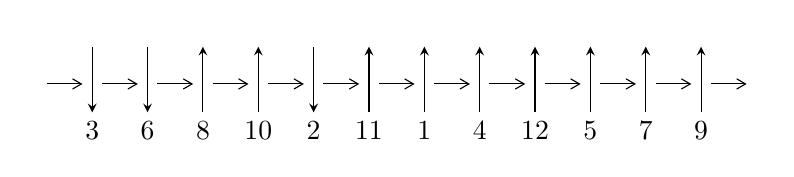
\begin{tikzpicture}[x=20pt, y=17pt]
	% nodes
	\node (C0) at (0, 0) {};
	\node (C1) at (1, 0) {};
	\node (C1U) at (1, +1) {};
	\node (C1D) at (1, -1) {3};

	\node (C2) at (2, 0) {};
	\node (C2U) at (2, +1) {};
	\node (C2D) at (2, -1) {6};

	\node (C3) at (3, 0) {};
	\node (C3U) at (3, +1) {};
	\node (C3D) at (3, -1) {8};

	\node (C4) at (4, 0) {};
	\node (C4U) at (4, +1) {};
	\node (C4D) at (4, -1) {10};

	\node (C5) at (5, 0) {};
	\node (C5U) at (5, +1) {};
	\node (C5D) at (5, -1) {2};

	\node (C6) at (6, 0) {};
	\node (C6U) at (6, +1) {};
	\node (C6D) at (6, -1) {11};

	\node (C7) at (7, 0) {};
	\node (C7U) at (7, +1) {};
	\node (C7D) at (7, -1) {1};

	\node (C8) at (8, 0) {};
	\node (C8U) at (8, +1) {};
	\node (C8D) at (8, -1) {4};

	\node (C9) at (9, 0) {};
	\node (C9U) at (9, +1) {};
	\node (C9D) at (9, -1) {12};

	\node (C10) at (10, 0) {};
	\node (C10U) at (10, +1) {};
	\node (C10D) at (10, -1) {5};

	\node (C11) at (11, 0) {};
	\node (C11U) at (11, +1) {};
	\node (C11D) at (11, -1) {7};

	\node (C12) at (12, 0) {};
	\node (C12U) at (12, +1) {};
	\node (C12D) at (12, -1) {9};
	\node (C13) at (13, 0) {};

	% arrows
	\draw[->,>={angle 60}]
	(C0) edge (C1) (C1) edge (C2) (C2) edge (C3) (C3) edge (C4) (C4) edge (C5) (C5) edge (C6) (C6) edge (C7) (C7) edge (C8) (C8) edge (C9) (C9) edge (C10) (C10) edge (C11) (C11) edge (C12) (C12) edge (C13) ;	\draw[->,>=stealth]
	(C1U) edge (C1D) (C2U) edge (C2D) (C3D) edge (C3U) (C4D) edge (C4U) (C5U) edge (C5D) (C6D) edge (C6U) (C7D) edge (C7U) (C8D) edge (C8U) (C9D) edge (C9U) (C10D) edge (C10U) (C11D) edge (C11U) (C12D) edge (C12U) ;
	\end{tikzpicture} \\
\hhline{~~} \\& 
\textbf{Solving Sequence} \\ \cline{2-2} 
 &
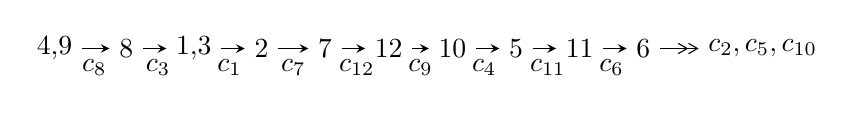
\begin{tikzpicture}[x=23pt, y=7pt]
	% node
	\node (A0) at (-1/8, 0) {4,9};
	\node (A1) at (1, 0) {8};
	\node (A2) at (33/16, 0) {1,3};
	\node (A3) at (25/8, 0) {2};
	\node (A4) at (33/8, 0) {7};
	\node (A5) at (41/8, 0) {12};
	\node (A6) at (49/8, 0) {10};
	\node (A7) at (57/8, 0) {5};
	\node (A8) at (65/8, 0) {11};
	\node (A9) at (73/8, 0) {6};
	\node (C1) at (1/2, -1) {$c_{8}$};
	\node (C2) at (3/2, -1) {$c_{3}$};
	\node (C3) at (21/8, -1) {$c_{1}$};
	\node (C4) at (29/8, -1) {$c_{7}$};
	\node (C5) at (37/8, -1) {$c_{12}$};
	\node (C6) at (45/8, -1) {$c_{9}$};
	\node (C7) at (53/8, -1) {$c_{4}$};
	\node (C8) at (61/8, -1) {$c_{11}$};
	\node (C9) at (69/8, -1) {$c_{6}$};
	\node (A10) at (11, 0) {$c_{2},c_{5},c_{10}$};

	% edge
	\draw[->,>=stealth]	
	(A0) edge (A1) (A1) edge (A2) (A2) edge (A3) (A3) edge (A4) (A4) edge (A5) (A5) edge (A6) (A6) edge (A7) (A7) edge (A8) (A8) edge (A9) ;
	\draw[->>,>={angle 60}]	
	(A9) edge (A10);
\end{tikzpicture} \\ 

\end{tabular} \\

\footnotetext{
The image of knot diagram is generated by the software ``\textbf{Draw programme}" developed by Andrew Bartholomew(\url{http://www.layer8.co.uk/maths/draw/index.htm\#Running-draw}), where we modified some parts for our purpose(\url{https://github.com/CATsTAILs/LinksPainter}).
}\phantom \\ \newline 
\centering \textbf{Ideals for irreducible components\footnotemark of $X_{\text{par}}$} 
 
\begin{align*}
I^u_{1}&=\langle 
3.17496\times10^{616} u^{134}+5.13470\times10^{616} u^{133}+\cdots+6.19398\times10^{616} b-1.62760\times10^{620},\\
\phantom{I^u_{1}}&\phantom{= \langle  }5.51099\times10^{619} u^{134}+1.88007\times10^{620} u^{133}+\cdots+3.10752\times10^{620} a-8.57469\times10^{623},\\
\phantom{I^u_{1}}&\phantom{= \langle  }u^{135}+u^{134}+\cdots+7750 u+5017\rangle \\
I^u_{2}&=\langle 
2.08927\times10^{22} u^{36}+2.56204\times10^{22} u^{35}+\cdots+7.67580\times10^{21} b+3.76326\times10^{22},\\
\phantom{I^u_{2}}&\phantom{= \langle  }-1.91416\times10^{21} u^{36}+1.69304\times10^{22} u^{35}+\cdots+7.67580\times10^{21} a+1.86496\times10^{22},\;u^{37}-12 u^{35}+\cdots- u-1\rangle \\
\\
\end{align*}
\raggedright * 2 irreducible components of $\dim_{\mathbb{C}}=0$, with total 172 representations.\\
\footnotetext{All coefficients of polynomials are rational numbers. But the coefficients are sometimes approximated in decimal forms when there is not enough margin.}
\newpage
\renewcommand{\arraystretch}{1}
\centering \section*{I. $I^u_{1}= \langle 3.17\times10^{616} u^{134}+5.13\times10^{616} u^{133}+\cdots+6.19\times10^{616} b-1.63\times10^{620},\;5.51\times10^{619} u^{134}+1.88\times10^{620} u^{133}+\cdots+3.11\times10^{620} a-8.57\times10^{623},\;u^{135}+u^{134}+\cdots+7750 u+5017 \rangle$}
\flushleft \textbf{(i) Arc colorings}\\
\begin{tabular}{m{7pt} m{180pt} m{7pt} m{180pt} }
\flushright $a_{4}=$&$\begin{pmatrix}0\\u\end{pmatrix}$ \\
\flushright $a_{9}=$&$\begin{pmatrix}1\\0\end{pmatrix}$ \\
\flushright $a_{8}=$&$\begin{pmatrix}1\\u^2\end{pmatrix}$ \\
\flushright $a_{1}=$&$\begin{pmatrix}-0.177344 u^{134}-0.605006 u^{133}+\cdots+5950.95 u+2759.34\\-0.512588 u^{134}-0.828983 u^{133}+\cdots+7681.07 u+2627.71\end{pmatrix}$ \\
\flushright $a_{3}=$&$\begin{pmatrix}- u\\- u^3+u\end{pmatrix}$ \\
\flushright $a_{2}=$&$\begin{pmatrix}0.263657 u^{134}+0.0494544 u^{133}+\cdots-169.075 u+811.076\\-0.628647 u^{134}-1.07304 u^{133}+\cdots+9934.28 u+3505.05\end{pmatrix}$ \\
\flushright $a_{7}=$&$\begin{pmatrix}-0.00826351 u^{134}+0.878969 u^{133}+\cdots-9133.12 u-5182.63\\-0.0243474 u^{134}-0.117595 u^{133}+\cdots+955.457 u+433.067\end{pmatrix}$ \\
\flushright $a_{12}=$&$\begin{pmatrix}0.335244 u^{134}+0.223977 u^{133}+\cdots-1730.12 u+131.626\\-0.512588 u^{134}-0.828983 u^{133}+\cdots+7681.07 u+2627.71\end{pmatrix}$ \\
\flushright $a_{10}=$&$\begin{pmatrix}-0.492155 u^{134}-0.951052 u^{133}+\cdots+8453.57 u+3107.01\\-0.933148 u^{134}-1.74478 u^{133}+\cdots+16041.9 u+5941.16\end{pmatrix}$ \\
\flushright $a_{5}=$&$\begin{pmatrix}0.646521 u^{134}+0.778334 u^{133}+\cdots-6570.11 u-1518.83\\0.661129 u^{134}+1.13677 u^{133}+\cdots-10388.5 u-3620.31\end{pmatrix}$ \\
\flushright $a_{11}=$&$\begin{pmatrix}-0.843358 u^{134}-0.644526 u^{133}+\cdots+4347.49 u-75.8403\\-0.455535 u^{134}-0.874228 u^{133}+\cdots+8006.36 u+3044.37\end{pmatrix}$ \\
\flushright $a_{6}=$&$\begin{pmatrix}0.593592 u^{134}+0.536821 u^{133}+\cdots-4315.52 u-495.398\\-0.347295 u^{134}-0.644904 u^{133}+\cdots+5736.93 u+2132.87\end{pmatrix}$\\&\end{tabular}
\flushleft \textbf{(ii) Obstruction class $= -1$}\\~\\
\flushleft \textbf{(iii) Cusp Shapes $= 1.96894 u^{134}+3.28735 u^{133}+\cdots-28454.3 u-9458.29$}\\~\\
\newpage\renewcommand{\arraystretch}{1}
\flushleft \textbf{(iv) u-Polynomials at the component}\newline \\
\begin{tabular}{m{50pt}|m{274pt}}
Crossings & \hspace{64pt}u-Polynomials at each crossing \\
\hline $$\begin{aligned}c_{1}\end{aligned}$$&$\begin{aligned}
&u^{135}+48 u^{134}+\cdots+4 u+1
\end{aligned}$\\
\hline $$\begin{aligned}c_{2},c_{5}\end{aligned}$$&$\begin{aligned}
&u^{135}+4 u^{134}+\cdots-18 u+1
\end{aligned}$\\
\hline $$\begin{aligned}c_{3},c_{8}\end{aligned}$$&$\begin{aligned}
&u^{135}+u^{134}+\cdots+7750 u+5017
\end{aligned}$\\
\hline $$\begin{aligned}c_{4},c_{10}\end{aligned}$$&$\begin{aligned}
&u^{135}- u^{134}+\cdots+5678572 u+1040987
\end{aligned}$\\
\hline $$\begin{aligned}c_{6},c_{11}\end{aligned}$$&$\begin{aligned}
&u^{135}+2 u^{134}+\cdots-535831 u-76529
\end{aligned}$\\
\hline $$\begin{aligned}c_{7}\end{aligned}$$&$\begin{aligned}
&u^{135}-2 u^{134}+\cdots-1565265 u-501775
\end{aligned}$\\
\hline $$\begin{aligned}c_{9},c_{12}\end{aligned}$$&$\begin{aligned}
&u^{135}+6 u^{134}+\cdots+26 u+1
\end{aligned}$\\
\hline
\end{tabular}\\~\\
\newpage\renewcommand{\arraystretch}{1}
\flushleft \textbf{(v) Riley Polynomials at the component}\newline \\
\begin{tabular}{m{50pt}|m{274pt}}
Crossings & \hspace{64pt}Riley Polynomials at each crossing \\
\hline $$\begin{aligned}c_{1}\end{aligned}$$&$\begin{aligned}
&y^{135}+92 y^{134}+\cdots+33596 y-1
\end{aligned}$\\
\hline $$\begin{aligned}c_{2},c_{5}\end{aligned}$$&$\begin{aligned}
&y^{135}-48 y^{134}+\cdots+4 y-1
\end{aligned}$\\
\hline $$\begin{aligned}c_{3},c_{8}\end{aligned}$$&$\begin{aligned}
&y^{135}-91 y^{134}+\cdots+1438372876 y-25170289
\end{aligned}$\\
\hline $$\begin{aligned}c_{4},c_{10}\end{aligned}$$&$\begin{aligned}
&y^{135}-119 y^{134}+\cdots+42184843029686 y-1083653934169
\end{aligned}$\\
\hline $$\begin{aligned}c_{6},c_{11}\end{aligned}$$&$\begin{aligned}
&y^{135}-98 y^{134}+\cdots+100193084177 y-5856687841
\end{aligned}$\\
\hline $$\begin{aligned}c_{7}\end{aligned}$$&$\begin{aligned}
&y^{135}-38 y^{134}+\cdots-6333962430975 y-251778150625
\end{aligned}$\\
\hline $$\begin{aligned}c_{9},c_{12}\end{aligned}$$&$\begin{aligned}
&y^{135}+74 y^{134}+\cdots+132 y-1
\end{aligned}$\\
\hline
\end{tabular}\\~\\
\newpage\flushleft \textbf{(vi) Complex Volumes and Cusp Shapes}
$$\begin{array}{c|c|c}  
\text{Solutions to }I^u_{1}& \I (\text{vol} + \sqrt{-1}CS) & \text{Cusp shape}\\
 \hline 
\begin{aligned}
u &= -0.954640 + 0.318925 I \\
a &= \phantom{-}1.022950 + 0.479534 I \\
b &= \phantom{-}0.409133 + 0.567557 I\end{aligned}
 & \phantom{-}0.43783 - 4.31705 I & \phantom{-0.000000 } 0 \\ \hline\begin{aligned}
u &= -0.954640 - 0.318925 I \\
a &= \phantom{-}1.022950 - 0.479534 I \\
b &= \phantom{-}0.409133 - 0.567557 I\end{aligned}
 & \phantom{-}0.43783 + 4.31705 I & \phantom{-0.000000 } 0 \\ \hline\begin{aligned}
u &= -1.016170 + 0.093526 I \\
a &= -0.504006 + 0.995437 I \\
b &= -0.27251 + 1.98430 I\end{aligned}
 & \phantom{-}2.61261 - 5.62917 I & \phantom{-0.000000 } 0 \\ \hline\begin{aligned}
u &= -1.016170 - 0.093526 I \\
a &= -0.504006 - 0.995437 I \\
b &= -0.27251 - 1.98430 I\end{aligned}
 & \phantom{-}2.61261 + 5.62917 I & \phantom{-0.000000 } 0 \\ \hline\begin{aligned}
u &= \phantom{-}1.021340 + 0.033322 I \\
a &= -0.966207 + 0.288532 I \\
b &= -0.44325 + 1.52596 I\end{aligned}
 & \phantom{-}1.64985 + 1.10466 I & \phantom{-0.000000 } 0 \\ \hline\begin{aligned}
u &= \phantom{-}1.021340 - 0.033322 I \\
a &= -0.966207 - 0.288532 I \\
b &= -0.44325 - 1.52596 I\end{aligned}
 & \phantom{-}1.64985 - 1.10466 I & \phantom{-0.000000 } 0 \\ \hline\begin{aligned}
u &= \phantom{-}0.045443 + 1.044390 I \\
a &= \phantom{-}0.206992 + 0.575475 I \\
b &= -0.153999 - 0.852553 I\end{aligned}
 & -2.34746 + 1.63033 I & \phantom{-0.000000 } 0 \\ \hline\begin{aligned}
u &= \phantom{-}0.045443 - 1.044390 I \\
a &= \phantom{-}0.206992 - 0.575475 I \\
b &= -0.153999 + 0.852553 I\end{aligned}
 & -2.34746 - 1.63033 I & \phantom{-0.000000 } 0 \\ \hline\begin{aligned}
u &= -1.053430 + 0.017888 I \\
a &= \phantom{-}1.96645 + 0.94497 I \\
b &= \phantom{-}0.407511 - 1.031440 I\end{aligned}
 & \phantom{-}8.16331 - 1.60493 I & \phantom{-0.000000 } 0 \\ \hline\begin{aligned}
u &= -1.053430 - 0.017888 I \\
a &= \phantom{-}1.96645 - 0.94497 I \\
b &= \phantom{-}0.407511 + 1.031440 I\end{aligned}
 & \phantom{-}8.16331 + 1.60493 I & \phantom{-0.000000 } 0\\
 \hline 
 \end{array}$$\newpage$$\begin{array}{c|c|c}  
\text{Solutions to }I^u_{1}& \I (\text{vol} + \sqrt{-1}CS) & \text{Cusp shape}\\
 \hline 
\begin{aligned}
u &= \phantom{-}0.366593 + 0.867646 I \\
a &= \phantom{-}0.021724 + 0.959308 I \\
b &= \phantom{-}0.609946 - 0.326417 I\end{aligned}
 & \phantom{-}6.32559 + 7.59825 I & \phantom{-0.000000 } 0 \\ \hline\begin{aligned}
u &= \phantom{-}0.366593 - 0.867646 I \\
a &= \phantom{-}0.021724 - 0.959308 I \\
b &= \phantom{-}0.609946 + 0.326417 I\end{aligned}
 & \phantom{-}6.32559 - 7.59825 I & \phantom{-0.000000 } 0 \\ \hline\begin{aligned}
u &= -0.340482 + 1.001910 I \\
a &= \phantom{-}0.0761110 + 0.0320509 I \\
b &= \phantom{-}0.577563 + 1.081620 I\end{aligned}
 & -1.49987 + 5.25116 I & \phantom{-0.000000 } 0 \\ \hline\begin{aligned}
u &= -0.340482 - 1.001910 I \\
a &= \phantom{-}0.0761110 - 0.0320509 I \\
b &= \phantom{-}0.577563 - 1.081620 I\end{aligned}
 & -1.49987 - 5.25116 I & \phantom{-0.000000 } 0 \\ \hline\begin{aligned}
u &= \phantom{-}0.926531 + 0.122035 I \\
a &= -1.022900 + 0.634029 I \\
b &= -0.949437 + 0.519992 I\end{aligned}
 & \phantom{-}0.989756 + 0.788732 I & \phantom{-0.000000 } 0 \\ \hline\begin{aligned}
u &= \phantom{-}0.926531 - 0.122035 I \\
a &= -1.022900 - 0.634029 I \\
b &= -0.949437 - 0.519992 I\end{aligned}
 & \phantom{-}0.989756 - 0.788732 I & \phantom{-0.000000 } 0 \\ \hline\begin{aligned}
u &= \phantom{-}0.981987 + 0.420245 I \\
a &= \phantom{-}0.107399 + 0.859771 I \\
b &= -0.331020 + 1.374450 I\end{aligned}
 & \phantom{-}2.10320 + 2.45744 I & \phantom{-0.000000 } 0 \\ \hline\begin{aligned}
u &= \phantom{-}0.981987 - 0.420245 I \\
a &= \phantom{-}0.107399 - 0.859771 I \\
b &= -0.331020 - 1.374450 I\end{aligned}
 & \phantom{-}2.10320 - 2.45744 I & \phantom{-0.000000 } 0 \\ \hline\begin{aligned}
u &= \phantom{-}1.075440 + 0.013274 I \\
a &= \phantom{-}1.144210 + 0.391008 I \\
b &= \phantom{-}0.340818 + 0.757547 I\end{aligned}
 & \phantom{-}1.85665 + 0.45415 I & \phantom{-0.000000 } 0 \\ \hline\begin{aligned}
u &= \phantom{-}1.075440 - 0.013274 I \\
a &= \phantom{-}1.144210 - 0.391008 I \\
b &= \phantom{-}0.340818 - 0.757547 I\end{aligned}
 & \phantom{-}1.85665 - 0.45415 I & \phantom{-0.000000 } 0\\
 \hline 
 \end{array}$$\newpage$$\begin{array}{c|c|c}  
\text{Solutions to }I^u_{1}& \I (\text{vol} + \sqrt{-1}CS) & \text{Cusp shape}\\
 \hline 
\begin{aligned}
u &= -0.328439 + 1.041220 I \\
a &= \phantom{-}0.323246 - 0.415650 I \\
b &= \phantom{-}0.115260 + 0.974194 I\end{aligned}
 & -3.71401 + 2.08606 I & \phantom{-0.000000 } 0 \\ \hline\begin{aligned}
u &= -0.328439 - 1.041220 I \\
a &= \phantom{-}0.323246 + 0.415650 I \\
b &= \phantom{-}0.115260 - 0.974194 I\end{aligned}
 & -3.71401 - 2.08606 I & \phantom{-0.000000 } 0 \\ \hline\begin{aligned}
u &= -0.978375 + 0.488563 I \\
a &= \phantom{-}1.44781 - 0.31474 I \\
b &= \phantom{-}0.315948 - 0.980472 I\end{aligned}
 & -3.56580 - 1.03017 I & \phantom{-0.000000 } 0 \\ \hline\begin{aligned}
u &= -0.978375 - 0.488563 I \\
a &= \phantom{-}1.44781 + 0.31474 I \\
b &= \phantom{-}0.315948 + 0.980472 I\end{aligned}
 & -3.56580 + 1.03017 I & \phantom{-0.000000 } 0 \\ \hline\begin{aligned}
u &= -0.800525 + 0.421653 I \\
a &= \phantom{-}0.599308 + 1.110760 I \\
b &= \phantom{-}0.89496 + 1.15377 I\end{aligned}
 & \phantom{-}1.63032 - 3.52071 I & \phantom{-0.000000 } 0 \\ \hline\begin{aligned}
u &= -0.800525 - 0.421653 I \\
a &= \phantom{-}0.599308 - 1.110760 I \\
b &= \phantom{-}0.89496 - 1.15377 I\end{aligned}
 & \phantom{-}1.63032 + 3.52071 I & \phantom{-0.000000 } 0 \\ \hline\begin{aligned}
u &= -0.803341 + 0.388664 I \\
a &= \phantom{-}1.06597 + 1.26585 I \\
b &= \phantom{-}0.477105 - 1.057170 I\end{aligned}
 & \phantom{-}5.47134 - 3.37942 I & \phantom{-0.000000 } 0 \\ \hline\begin{aligned}
u &= -0.803341 - 0.388664 I \\
a &= \phantom{-}1.06597 - 1.26585 I \\
b &= \phantom{-}0.477105 + 1.057170 I\end{aligned}
 & \phantom{-}5.47134 + 3.37942 I & \phantom{-0.000000 } 0 \\ \hline\begin{aligned}
u &= \phantom{-}1.060180 + 0.351103 I \\
a &= \phantom{-}1.93172 + 0.28529 I \\
b &= \phantom{-}1.17905 + 1.23783 I\end{aligned}
 & \phantom{-}6.39857 + 5.83677 I & \phantom{-0.000000 } 0 \\ \hline\begin{aligned}
u &= \phantom{-}1.060180 - 0.351103 I \\
a &= \phantom{-}1.93172 - 0.28529 I \\
b &= \phantom{-}1.17905 - 1.23783 I\end{aligned}
 & \phantom{-}6.39857 - 5.83677 I & \phantom{-0.000000 } 0\\
 \hline 
 \end{array}$$\newpage$$\begin{array}{c|c|c}  
\text{Solutions to }I^u_{1}& \I (\text{vol} + \sqrt{-1}CS) & \text{Cusp shape}\\
 \hline 
\begin{aligned}
u &= -0.498013 + 0.702051 I \\
a &= -0.354922 - 0.896451 I \\
b &= \phantom{-}0.580572 + 0.322418 I\end{aligned}
 & \phantom{-}7.64173 - 1.70956 I & \phantom{-0.000000 } 0 \\ \hline\begin{aligned}
u &= -0.498013 - 0.702051 I \\
a &= -0.354922 + 0.896451 I \\
b &= \phantom{-}0.580572 - 0.322418 I\end{aligned}
 & \phantom{-}7.64173 + 1.70956 I & \phantom{-0.000000 } 0 \\ \hline\begin{aligned}
u &= -1.129260 + 0.169822 I \\
a &= -1.45636 + 0.25196 I \\
b &= -0.65385 + 1.34140 I\end{aligned}
 & \phantom{-}3.05271 - 5.01411 I & \phantom{-0.000000 } 0 \\ \hline\begin{aligned}
u &= -1.129260 - 0.169822 I \\
a &= -1.45636 - 0.25196 I \\
b &= -0.65385 - 1.34140 I\end{aligned}
 & \phantom{-}3.05271 + 5.01411 I & \phantom{-0.000000 } 0 \\ \hline\begin{aligned}
u &= \phantom{-}1.155020 + 0.033424 I \\
a &= \phantom{-}1.94958 - 0.72796 I \\
b &= \phantom{-}0.403614 + 1.012110 I\end{aligned}
 & \phantom{-}7.77279 + 6.93659 I & \phantom{-0.000000 } 0 \\ \hline\begin{aligned}
u &= \phantom{-}1.155020 - 0.033424 I \\
a &= \phantom{-}1.94958 + 0.72796 I \\
b &= \phantom{-}0.403614 - 1.012110 I\end{aligned}
 & \phantom{-}7.77279 - 6.93659 I & \phantom{-0.000000 } 0 \\ \hline\begin{aligned}
u &= -0.545023 + 0.637806 I \\
a &= \phantom{-}0.042747 - 0.188833 I \\
b &= \phantom{-}0.022084 + 1.256470 I\end{aligned}
 & -5.04744 - 3.41143 I & \phantom{-0.000000 } 0 \\ \hline\begin{aligned}
u &= -0.545023 - 0.637806 I \\
a &= \phantom{-}0.042747 + 0.188833 I \\
b &= \phantom{-}0.022084 - 1.256470 I\end{aligned}
 & -5.04744 + 3.41143 I & \phantom{-0.000000 } 0 \\ \hline\begin{aligned}
u &= \phantom{-}0.834362 + 0.002369 I \\
a &= -2.38438 - 0.35600 I \\
b &= -0.971622 - 0.629846 I\end{aligned}
 & \phantom{-}0.078046 - 0.408426 I & \phantom{-0.000000 } 0 \\ \hline\begin{aligned}
u &= \phantom{-}0.834362 - 0.002369 I \\
a &= -2.38438 + 0.35600 I \\
b &= -0.971622 + 0.629846 I\end{aligned}
 & \phantom{-}0.078046 + 0.408426 I & \phantom{-0.000000 } 0\\
 \hline 
 \end{array}$$\newpage$$\begin{array}{c|c|c}  
\text{Solutions to }I^u_{1}& \I (\text{vol} + \sqrt{-1}CS) & \text{Cusp shape}\\
 \hline 
\begin{aligned}
u &= -0.818052 + 0.120704 I \\
a &= -1.74314 - 1.47278 I \\
b &= \phantom{-}0.125304 - 0.347815 I\end{aligned}
 & \phantom{-}7.31926 - 1.58600 I & \phantom{-0.000000 } 0 \\ \hline\begin{aligned}
u &= -0.818052 - 0.120704 I \\
a &= -1.74314 + 1.47278 I \\
b &= \phantom{-}0.125304 + 0.347815 I\end{aligned}
 & \phantom{-}7.31926 + 1.58600 I & \phantom{-0.000000 } 0 \\ \hline\begin{aligned}
u &= \phantom{-}1.086350 + 0.476264 I \\
a &= -1.29461 + 0.78264 I \\
b &= -0.646687 - 0.048956 I\end{aligned}
 & \phantom{-}5.92842 + 6.96503 I & \phantom{-0.000000 } 0 \\ \hline\begin{aligned}
u &= \phantom{-}1.086350 - 0.476264 I \\
a &= -1.29461 - 0.78264 I \\
b &= -0.646687 + 0.048956 I\end{aligned}
 & \phantom{-}5.92842 - 6.96503 I & \phantom{-0.000000 } 0 \\ \hline\begin{aligned}
u &= \phantom{-}0.776366 + 0.241907 I \\
a &= -1.93972 + 1.89576 I \\
b &= \phantom{-}0.004136 + 0.356197 I\end{aligned}
 & \phantom{-}5.99324 + 7.26808 I & \phantom{-0.000000 } 0 \\ \hline\begin{aligned}
u &= \phantom{-}0.776366 - 0.241907 I \\
a &= -1.93972 - 1.89576 I \\
b &= \phantom{-}0.004136 - 0.356197 I\end{aligned}
 & \phantom{-}5.99324 - 7.26808 I & \phantom{-0.000000 } 0 \\ \hline\begin{aligned}
u &= -0.017793 + 1.188140 I \\
a &= \phantom{-}0.150013 + 0.321516 I \\
b &= \phantom{-}0.558235 - 1.096620 I\end{aligned}
 & \phantom{-}5.47564 - 6.37114 I & \phantom{-0.000000 } 0 \\ \hline\begin{aligned}
u &= -0.017793 - 1.188140 I \\
a &= \phantom{-}0.150013 - 0.321516 I \\
b &= \phantom{-}0.558235 + 1.096620 I\end{aligned}
 & \phantom{-}5.47564 + 6.37114 I & \phantom{-0.000000 } 0 \\ \hline\begin{aligned}
u &= \phantom{-}0.085695 + 0.805479 I \\
a &= \phantom{-}0.162751 + 0.609323 I \\
b &= -0.144643 - 1.008910 I\end{aligned}
 & -2.21134 + 1.64026 I & \phantom{-0.000000 } 0 \\ \hline\begin{aligned}
u &= \phantom{-}0.085695 - 0.805479 I \\
a &= \phantom{-}0.162751 - 0.609323 I \\
b &= -0.144643 + 1.008910 I\end{aligned}
 & -2.21134 - 1.64026 I & \phantom{-0.000000 } 0\\
 \hline 
 \end{array}$$\newpage$$\begin{array}{c|c|c}  
\text{Solutions to }I^u_{1}& \I (\text{vol} + \sqrt{-1}CS) & \text{Cusp shape}\\
 \hline 
\begin{aligned}
u &= \phantom{-}1.146760 + 0.343908 I \\
a &= -1.62910 - 0.73914 I \\
b &= -0.572216 - 1.071540 I\end{aligned}
 & -1.66219 + 5.65655 I & \phantom{-0.000000 } 0 \\ \hline\begin{aligned}
u &= \phantom{-}1.146760 - 0.343908 I \\
a &= -1.62910 + 0.73914 I \\
b &= -0.572216 + 1.071540 I\end{aligned}
 & -1.66219 - 5.65655 I & \phantom{-0.000000 } 0 \\ \hline\begin{aligned}
u &= \phantom{-}0.073056 + 0.799254 I \\
a &= -0.696832 - 0.588441 I \\
b &= -0.354850 + 1.227410 I\end{aligned}
 & -0.84591 - 6.66630 I & \phantom{-0.000000 } 0 \\ \hline\begin{aligned}
u &= \phantom{-}0.073056 - 0.799254 I \\
a &= -0.696832 + 0.588441 I \\
b &= -0.354850 - 1.227410 I\end{aligned}
 & -0.84591 + 6.66630 I & \phantom{-0.000000 } 0 \\ \hline\begin{aligned}
u &= -1.199230 + 0.037550 I \\
a &= -1.075130 + 0.804898 I \\
b &= -0.75485 + 1.21965 I\end{aligned}
 & \phantom{-}3.47495 - 4.36587 I & \phantom{-0.000000 } 0 \\ \hline\begin{aligned}
u &= -1.199230 - 0.037550 I \\
a &= -1.075130 - 0.804898 I \\
b &= -0.75485 - 1.21965 I\end{aligned}
 & \phantom{-}3.47495 + 4.36587 I & \phantom{-0.000000 } 0 \\ \hline\begin{aligned}
u &= -1.204740 + 0.210079 I \\
a &= -0.273983 + 0.754365 I \\
b &= \phantom{-}0.376121 + 0.529314 I\end{aligned}
 & \phantom{-}7.21042 + 0.43135 I & \phantom{-0.000000 } 0 \\ \hline\begin{aligned}
u &= -1.204740 - 0.210079 I \\
a &= -0.273983 - 0.754365 I \\
b &= \phantom{-}0.376121 - 0.529314 I\end{aligned}
 & \phantom{-}7.21042 - 0.43135 I & \phantom{-0.000000 } 0 \\ \hline\begin{aligned}
u &= -1.181180 + 0.337932 I \\
a &= -1.36591 - 0.54634 I \\
b &= -0.743455 + 0.035130 I\end{aligned}
 & \phantom{-}6.99082 - 1.16731 I & \phantom{-0.000000 } 0 \\ \hline\begin{aligned}
u &= -1.181180 - 0.337932 I \\
a &= -1.36591 + 0.54634 I \\
b &= -0.743455 - 0.035130 I\end{aligned}
 & \phantom{-}6.99082 + 1.16731 I & \phantom{-0.000000 } 0\\
 \hline 
 \end{array}$$\newpage$$\begin{array}{c|c|c}  
\text{Solutions to }I^u_{1}& \I (\text{vol} + \sqrt{-1}CS) & \text{Cusp shape}\\
 \hline 
\begin{aligned}
u &= \phantom{-}0.618926 + 1.061280 I \\
a &= \phantom{-}0.190901 - 0.125372 I \\
b &= -0.350949 + 1.005310 I\end{aligned}
 & -3.33552 - 0.69088 I & \phantom{-0.000000 } 0 \\ \hline\begin{aligned}
u &= \phantom{-}0.618926 - 1.061280 I \\
a &= \phantom{-}0.190901 + 0.125372 I \\
b &= -0.350949 - 1.005310 I\end{aligned}
 & -3.33552 + 0.69088 I & \phantom{-0.000000 } 0 \\ \hline\begin{aligned}
u &= \phantom{-}0.085830 + 0.757982 I \\
a &= -0.707780 + 0.757507 I \\
b &= -0.364628 - 1.172950 I\end{aligned}
 & -0.46524 + 1.51647 I & \phantom{-0.000000 } 0 \\ \hline\begin{aligned}
u &= \phantom{-}0.085830 - 0.757982 I \\
a &= -0.707780 - 0.757507 I \\
b &= -0.364628 + 1.172950 I\end{aligned}
 & -0.46524 - 1.51647 I & \phantom{-0.000000 } 0 \\ \hline\begin{aligned}
u &= \phantom{-}0.110124 + 0.751924 I \\
a &= -0.506523 + 0.036217 I \\
b &= -0.784393 + 0.029656 I\end{aligned}
 & \phantom{-}3.03685 - 2.59231 I & \phantom{-0.000000 } 0 \\ \hline\begin{aligned}
u &= \phantom{-}0.110124 - 0.751924 I \\
a &= -0.506523 - 0.036217 I \\
b &= -0.784393 - 0.029656 I\end{aligned}
 & \phantom{-}3.03685 + 2.59231 I & \phantom{-0.000000 } 0 \\ \hline\begin{aligned}
u &= \phantom{-}1.099620 + 0.592482 I \\
a &= -1.343520 + 0.130959 I \\
b &= -0.616344 - 1.192720 I\end{aligned}
 & -1.52443 + 6.62250 I & \phantom{-0.000000 } 0 \\ \hline\begin{aligned}
u &= \phantom{-}1.099620 - 0.592482 I \\
a &= -1.343520 - 0.130959 I \\
b &= -0.616344 + 1.192720 I\end{aligned}
 & -1.52443 - 6.62250 I & \phantom{-0.000000 } 0 \\ \hline\begin{aligned}
u &= -0.670835 + 0.267149 I \\
a &= \phantom{-}1.03893 - 1.55456 I \\
b &= \phantom{-}0.16201 - 1.42363 I\end{aligned}
 & \phantom{-}1.97161 + 4.17594 I & \phantom{-0.000000 } 0 \\ \hline\begin{aligned}
u &= -0.670835 - 0.267149 I \\
a &= \phantom{-}1.03893 + 1.55456 I \\
b &= \phantom{-}0.16201 + 1.42363 I\end{aligned}
 & \phantom{-}1.97161 - 4.17594 I & \phantom{-0.000000 } 0\\
 \hline 
 \end{array}$$\newpage$$\begin{array}{c|c|c}  
\text{Solutions to }I^u_{1}& \I (\text{vol} + \sqrt{-1}CS) & \text{Cusp shape}\\
 \hline 
\begin{aligned}
u &= \phantom{-}1.248030 + 0.339213 I \\
a &= \phantom{-}1.35352 - 0.53397 I \\
b &= \phantom{-}0.463130 + 0.981232 I\end{aligned}
 & \phantom{-}4.16663 + 2.76856 I & \phantom{-0.000000 } 0 \\ \hline\begin{aligned}
u &= \phantom{-}1.248030 - 0.339213 I \\
a &= \phantom{-}1.35352 + 0.53397 I \\
b &= \phantom{-}0.463130 - 0.981232 I\end{aligned}
 & \phantom{-}4.16663 - 2.76856 I & \phantom{-0.000000 } 0 \\ \hline\begin{aligned}
u &= -0.057520 + 1.305510 I \\
a &= \phantom{-}0.221046 - 0.269379 I \\
b &= \phantom{-}0.556090 + 1.097680 I\end{aligned}
 & \phantom{-}4.16357 + 12.28470 I & \phantom{-0.000000 } 0 \\ \hline\begin{aligned}
u &= -0.057520 - 1.305510 I \\
a &= \phantom{-}0.221046 + 0.269379 I \\
b &= \phantom{-}0.556090 - 1.097680 I\end{aligned}
 & \phantom{-}4.16357 - 12.28470 I & \phantom{-0.000000 } 0 \\ \hline\begin{aligned}
u &= -1.166530 + 0.590664 I \\
a &= \phantom{-}1.62830 - 0.01371 I \\
b &= \phantom{-}0.86405 - 1.15542 I\end{aligned}
 & \phantom{-}1.10197 - 10.93990 I & \phantom{-0.000000 } 0 \\ \hline\begin{aligned}
u &= -1.166530 - 0.590664 I \\
a &= \phantom{-}1.62830 + 0.01371 I \\
b &= \phantom{-}0.86405 + 1.15542 I\end{aligned}
 & \phantom{-}1.10197 + 10.93990 I & \phantom{-0.000000 } 0 \\ \hline\begin{aligned}
u &= -1.31941\phantom{ +0.000000I} \\
a &= -1.26332\phantom{ +0.000000I} \\
b &= -0.929967\phantom{ +0.000000I}\end{aligned}
 & \phantom{-}5.55269\phantom{ +0.000000I} & \phantom{-0.000000 } 0 \\ \hline\begin{aligned}
u &= \phantom{-}1.249810 + 0.423782 I \\
a &= \phantom{-}1.310290 + 0.187469 I \\
b &= \phantom{-}0.396114 + 0.914800 I\end{aligned}
 & \phantom{-}1.36572 + 2.83945 I & \phantom{-0.000000 } 0 \\ \hline\begin{aligned}
u &= \phantom{-}1.249810 - 0.423782 I \\
a &= \phantom{-}1.310290 - 0.187469 I \\
b &= \phantom{-}0.396114 - 0.914800 I\end{aligned}
 & \phantom{-}1.36572 - 2.83945 I & \phantom{-0.000000 } 0 \\ \hline\begin{aligned}
u &= -1.298070 + 0.296134 I \\
a &= -1.360160 + 0.280784 I \\
b &= -0.604488 + 1.211900 I\end{aligned}
 & \phantom{-}2.15466 - 5.46034 I & \phantom{-0.000000 } 0\\
 \hline 
 \end{array}$$\newpage$$\begin{array}{c|c|c}  
\text{Solutions to }I^u_{1}& \I (\text{vol} + \sqrt{-1}CS) & \text{Cusp shape}\\
 \hline 
\begin{aligned}
u &= -1.298070 - 0.296134 I \\
a &= -1.360160 - 0.280784 I \\
b &= -0.604488 - 1.211900 I\end{aligned}
 & \phantom{-}2.15466 + 5.46034 I & \phantom{-0.000000 } 0 \\ \hline\begin{aligned}
u &= \phantom{-}1.300800 + 0.307473 I \\
a &= \phantom{-}1.329500 - 0.451366 I \\
b &= \phantom{-}1.38709 - 0.42975 I\end{aligned}
 & \phantom{-}12.73450 + 5.05687 I & \phantom{-0.000000 } 0 \\ \hline\begin{aligned}
u &= \phantom{-}1.300800 - 0.307473 I \\
a &= \phantom{-}1.329500 + 0.451366 I \\
b &= \phantom{-}1.38709 + 0.42975 I\end{aligned}
 & \phantom{-}12.73450 - 5.05687 I & \phantom{-0.000000 } 0 \\ \hline\begin{aligned}
u &= \phantom{-}1.298880 + 0.423032 I \\
a &= -1.82059 - 0.41547 I \\
b &= -0.498197 - 1.136970 I\end{aligned}
 & \phantom{-}3.02034 + 11.19720 I & \phantom{-0.000000 } 0 \\ \hline\begin{aligned}
u &= \phantom{-}1.298880 - 0.423032 I \\
a &= -1.82059 + 0.41547 I \\
b &= -0.498197 + 1.136970 I\end{aligned}
 & \phantom{-}3.02034 - 11.19720 I & \phantom{-0.000000 } 0 \\ \hline\begin{aligned}
u &= -1.317950 + 0.373625 I \\
a &= -1.72566 + 0.35705 I \\
b &= -0.512546 + 1.160790 I\end{aligned}
 & \phantom{-}3.88460 - 5.67759 I & \phantom{-0.000000 } 0 \\ \hline\begin{aligned}
u &= -1.317950 - 0.373625 I \\
a &= -1.72566 - 0.35705 I \\
b &= -0.512546 - 1.160790 I\end{aligned}
 & \phantom{-}3.88460 + 5.67759 I & \phantom{-0.000000 } 0 \\ \hline\begin{aligned}
u &= \phantom{-}0.622354 + 0.045822 I \\
a &= -0.436758 - 1.255640 I \\
b &= -0.525781 - 0.579751 I\end{aligned}
 & \phantom{-}0.979130 - 0.632124 I & \phantom{-}9.84605 + 0. I\phantom{ +0.000000I} \\ \hline\begin{aligned}
u &= \phantom{-}0.622354 - 0.045822 I \\
a &= -0.436758 + 1.255640 I \\
b &= -0.525781 + 0.579751 I\end{aligned}
 & \phantom{-}0.979130 + 0.632124 I & \phantom{-}9.84605 + 0. I\phantom{ +0.000000I} \\ \hline\begin{aligned}
u &= -1.344500 + 0.385467 I \\
a &= \phantom{-}1.225180 + 0.422218 I \\
b &= \phantom{-}1.276030 + 0.388643 I\end{aligned}
 & \phantom{-}11.3606 - 11.9126 I & \phantom{-0.000000 } 0\\
 \hline 
 \end{array}$$\newpage$$\begin{array}{c|c|c}  
\text{Solutions to }I^u_{1}& \I (\text{vol} + \sqrt{-1}CS) & \text{Cusp shape}\\
 \hline 
\begin{aligned}
u &= -1.344500 - 0.385467 I \\
a &= \phantom{-}1.225180 - 0.422218 I \\
b &= \phantom{-}1.276030 - 0.388643 I\end{aligned}
 & \phantom{-}11.3606 + 11.9126 I & \phantom{-0.000000 } 0 \\ \hline\begin{aligned}
u &= -1.282610 + 0.561653 I \\
a &= \phantom{-}1.357460 - 0.132402 I \\
b &= \phantom{-}0.420339 - 0.943750 I\end{aligned}
 & -0.49644 - 7.87026 I & \phantom{-0.000000 } 0 \\ \hline\begin{aligned}
u &= -1.282610 - 0.561653 I \\
a &= \phantom{-}1.357460 + 0.132402 I \\
b &= \phantom{-}0.420339 + 0.943750 I\end{aligned}
 & -0.49644 + 7.87026 I & \phantom{-0.000000 } 0 \\ \hline\begin{aligned}
u &= -1.409590 + 0.028451 I \\
a &= \phantom{-}0.37037 - 1.41879 I \\
b &= \phantom{-}0.297929 - 0.666588 I\end{aligned}
 & \phantom{-}9.53256 - 1.57438 I & \phantom{-0.000000 } 0 \\ \hline\begin{aligned}
u &= -1.409590 - 0.028451 I \\
a &= \phantom{-}0.37037 + 1.41879 I \\
b &= \phantom{-}0.297929 + 0.666588 I\end{aligned}
 & \phantom{-}9.53256 + 1.57438 I & \phantom{-0.000000 } 0 \\ \hline\begin{aligned}
u &= -1.42409 + 0.21233 I \\
a &= -1.030960 - 0.005193 I \\
b &= -0.977527 - 0.165450 I\end{aligned}
 & \phantom{-}7.65750 - 0.58902 I & \phantom{-0.000000 } 0 \\ \hline\begin{aligned}
u &= -1.42409 - 0.21233 I \\
a &= -1.030960 + 0.005193 I \\
b &= -0.977527 + 0.165450 I\end{aligned}
 & \phantom{-}7.65750 + 0.58902 I & \phantom{-0.000000 } 0 \\ \hline\begin{aligned}
u &= \phantom{-}1.40629 + 0.32566 I \\
a &= -0.975854 + 0.040849 I \\
b &= -0.975841 + 0.187470 I\end{aligned}
 & \phantom{-}6.80870 + 6.30526 I & \phantom{-0.000000 } 0 \\ \hline\begin{aligned}
u &= \phantom{-}1.40629 - 0.32566 I \\
a &= -0.975854 - 0.040849 I \\
b &= -0.975841 - 0.187470 I\end{aligned}
 & \phantom{-}6.80870 - 6.30526 I & \phantom{-0.000000 } 0 \\ \hline\begin{aligned}
u &= \phantom{-}0.269153 + 0.476261 I \\
a &= -0.944603 - 0.688052 I \\
b &= \phantom{-}0.588619 - 1.176620 I\end{aligned}
 & \phantom{-}4.17085 - 2.44633 I & \phantom{-}8.78478 + 2.14755 I\\
 \hline 
 \end{array}$$\newpage$$\begin{array}{c|c|c}  
\text{Solutions to }I^u_{1}& \I (\text{vol} + \sqrt{-1}CS) & \text{Cusp shape}\\
 \hline 
\begin{aligned}
u &= \phantom{-}0.269153 - 0.476261 I \\
a &= -0.944603 + 0.688052 I \\
b &= \phantom{-}0.588619 + 1.176620 I\end{aligned}
 & \phantom{-}4.17085 + 2.44633 I & \phantom{-}8.78478 - 2.14755 I \\ \hline\begin{aligned}
u &= -1.22598 + 0.81052 I \\
a &= \phantom{-}0.826768 + 0.544146 I \\
b &= \phantom{-}0.541901 - 1.003310 I\end{aligned}
 & \phantom{-}9.23685 - 4.51705 I & \phantom{-0.000000 } 0 \\ \hline\begin{aligned}
u &= -1.22598 - 0.81052 I \\
a &= \phantom{-}0.826768 - 0.544146 I \\
b &= \phantom{-}0.541901 + 1.003310 I\end{aligned}
 & \phantom{-}9.23685 + 4.51705 I & \phantom{-0.000000 } 0 \\ \hline\begin{aligned}
u &= \phantom{-}1.47023 + 0.01762 I \\
a &= \phantom{-}0.59650 + 1.32725 I \\
b &= \phantom{-}0.314668 + 0.696933 I\end{aligned}
 & \phantom{-}8.95415 - 3.75498 I & \phantom{-0.000000 } 0 \\ \hline\begin{aligned}
u &= \phantom{-}1.47023 - 0.01762 I \\
a &= \phantom{-}0.59650 - 1.32725 I \\
b &= \phantom{-}0.314668 - 0.696933 I\end{aligned}
 & \phantom{-}8.95415 + 3.75498 I & \phantom{-0.000000 } 0 \\ \hline\begin{aligned}
u &= -0.224340 + 0.467691 I \\
a &= \phantom{-}1.207990 + 0.536436 I \\
b &= \phantom{-}0.160603 + 0.050600 I\end{aligned}
 & -1.54497 + 0.95371 I & -0.72705 - 2.44882 I \\ \hline\begin{aligned}
u &= -0.224340 - 0.467691 I \\
a &= \phantom{-}1.207990 - 0.536436 I \\
b &= \phantom{-}0.160603 - 0.050600 I\end{aligned}
 & -1.54497 - 0.95371 I & -0.72705 + 2.44882 I \\ \hline\begin{aligned}
u &= \phantom{-}0.518137\phantom{ +0.000000I} \\
a &= -4.13492\phantom{ +0.000000I} \\
b &= \phantom{-}0.0908048\phantom{ +0.000000I}\end{aligned}
 & \phantom{-}1.00231\phantom{ +0.000000I} & -0.767990\phantom{ +0.000000I} \\ \hline\begin{aligned}
u &= \phantom{-}1.38332 + 0.55183 I \\
a &= \phantom{-}1.44512 + 0.08441 I \\
b &= \phantom{-}0.76996 + 1.29547 I\end{aligned}
 & \phantom{-}9.8865 + 12.4224 I & \phantom{-0.000000 } 0 \\ \hline\begin{aligned}
u &= \phantom{-}1.38332 - 0.55183 I \\
a &= \phantom{-}1.44512 - 0.08441 I \\
b &= \phantom{-}0.76996 - 1.29547 I\end{aligned}
 & \phantom{-}9.8865 - 12.4224 I & \phantom{-0.000000 } 0\\
 \hline 
 \end{array}$$\newpage$$\begin{array}{c|c|c}  
\text{Solutions to }I^u_{1}& \I (\text{vol} + \sqrt{-1}CS) & \text{Cusp shape}\\
 \hline 
\begin{aligned}
u &= -0.26803 + 1.46651 I \\
a &= -0.014028 + 0.375503 I \\
b &= -0.398119 - 0.851557 I\end{aligned}
 & \phantom{-}0.198012 - 0.942296 I & \phantom{-0.000000 } 0 \\ \hline\begin{aligned}
u &= -0.26803 - 1.46651 I \\
a &= -0.014028 - 0.375503 I \\
b &= -0.398119 + 0.851557 I\end{aligned}
 & \phantom{-}0.198012 + 0.942296 I & \phantom{-0.000000 } 0 \\ \hline\begin{aligned}
u &= -0.406108 + 0.254970 I \\
a &= \phantom{-}3.23976 + 1.32405 I \\
b &= \phantom{-}1.045350 - 0.273646 I\end{aligned}
 & \phantom{-}0.658119 + 0.043507 I & \phantom{-}6.16916 + 1.22417 I \\ \hline\begin{aligned}
u &= -0.406108 - 0.254970 I \\
a &= \phantom{-}3.23976 - 1.32405 I \\
b &= \phantom{-}1.045350 + 0.273646 I\end{aligned}
 & \phantom{-}0.658119 - 0.043507 I & \phantom{-}6.16916 - 1.22417 I \\ \hline\begin{aligned}
u &= \phantom{-}0.351894 + 0.324168 I \\
a &= -0.552806 - 0.277941 I \\
b &= -0.269642 + 1.323580 I\end{aligned}
 & -4.34526 - 2.61796 I & \phantom{-}3.76862 - 10.99788 I \\ \hline\begin{aligned}
u &= \phantom{-}0.351894 - 0.324168 I \\
a &= -0.552806 + 0.277941 I \\
b &= -0.269642 - 1.323580 I\end{aligned}
 & -4.34526 + 2.61796 I & \phantom{-}3.76862 + 10.99788 I \\ \hline\begin{aligned}
u &= \phantom{-}0.41133 + 1.46911 I \\
a &= -0.013847 - 0.308079 I \\
b &= -0.415500 + 0.890485 I\end{aligned}
 & \phantom{-}0.04370 - 4.35843 I & \phantom{-0.000000 } 0 \\ \hline\begin{aligned}
u &= \phantom{-}0.41133 - 1.46911 I \\
a &= -0.013847 + 0.308079 I \\
b &= -0.415500 - 0.890485 I\end{aligned}
 & \phantom{-}0.04370 + 4.35843 I & \phantom{-0.000000 } 0 \\ \hline\begin{aligned}
u &= -1.41128 + 0.60551 I \\
a &= \phantom{-}1.42796 - 0.04215 I \\
b &= \phantom{-}0.73715 - 1.28137 I\end{aligned}
 & \phantom{-}8.4921 - 18.9052 I & \phantom{-0.000000 } 0 \\ \hline\begin{aligned}
u &= -1.41128 - 0.60551 I \\
a &= \phantom{-}1.42796 + 0.04215 I \\
b &= \phantom{-}0.73715 + 1.28137 I\end{aligned}
 & \phantom{-}8.4921 + 18.9052 I & \phantom{-0.000000 } 0\\
 \hline 
 \end{array}$$\newpage$$\begin{array}{c|c|c}  
\text{Solutions to }I^u_{1}& \I (\text{vol} + \sqrt{-1}CS) & \text{Cusp shape}\\
 \hline 
\begin{aligned}
u &= \phantom{-}1.52830 + 0.15956 I \\
a &= \phantom{-}0.497251 - 0.699857 I \\
b &= \phantom{-}0.420813 - 0.679037 I\end{aligned}
 & \phantom{-}5.19359 - 0.98092 I & \phantom{-0.000000 } 0 \\ \hline\begin{aligned}
u &= \phantom{-}1.52830 - 0.15956 I \\
a &= \phantom{-}0.497251 + 0.699857 I \\
b &= \phantom{-}0.420813 + 0.679037 I\end{aligned}
 & \phantom{-}5.19359 + 0.98092 I & \phantom{-0.000000 } 0 \\ \hline\begin{aligned}
u &= \phantom{-}1.34454 + 0.74655 I \\
a &= \phantom{-}0.880057 - 0.467093 I \\
b &= \phantom{-}0.540708 + 0.983870 I\end{aligned}
 & \phantom{-}8.85975 - 1.11909 I & \phantom{-0.000000 } 0 \\ \hline\begin{aligned}
u &= \phantom{-}1.34454 - 0.74655 I \\
a &= \phantom{-}0.880057 + 0.467093 I \\
b &= \phantom{-}0.540708 - 0.983870 I\end{aligned}
 & \phantom{-}8.85975 + 1.11909 I & \phantom{-0.000000 } 0 \\ \hline\begin{aligned}
u &= -1.45178 + 0.59117 I \\
a &= -1.112410 + 0.007592 I \\
b &= -0.614404 + 1.221490 I\end{aligned}
 & \phantom{-}4.55748 - 6.26390 I & \phantom{-0.000000 } 0 \\ \hline\begin{aligned}
u &= -1.45178 - 0.59117 I \\
a &= -1.112410 - 0.007592 I \\
b &= -0.614404 - 1.221490 I\end{aligned}
 & \phantom{-}4.55748 + 6.26390 I & \phantom{-0.000000 } 0 \\ \hline\begin{aligned}
u &= \phantom{-}1.43211 + 0.69162 I \\
a &= -1.105450 + 0.054070 I \\
b &= -0.609416 - 1.221970 I\end{aligned}
 & \phantom{-}3.73815 + 11.96640 I & \phantom{-0.000000 } 0 \\ \hline\begin{aligned}
u &= \phantom{-}1.43211 - 0.69162 I \\
a &= -1.105450 - 0.054070 I \\
b &= -0.609416 + 1.221970 I\end{aligned}
 & \phantom{-}3.73815 - 11.96640 I & \phantom{-0.000000 } 0 \\ \hline\begin{aligned}
u &= -0.386930 + 0.064980 I \\
a &= \phantom{-}1.19259 + 2.50460 I \\
b &= -0.287333 + 0.718290 I\end{aligned}
 & \phantom{-}0.74093 - 3.92926 I & \phantom{-}9.27224 + 7.12527 I \\ \hline\begin{aligned}
u &= -0.386930 - 0.064980 I \\
a &= \phantom{-}1.19259 - 2.50460 I \\
b &= -0.287333 - 0.718290 I\end{aligned}
 & \phantom{-}0.74093 + 3.92926 I & \phantom{-}9.27224 - 7.12527 I\\
 \hline 
 \end{array}$$\newpage$$\begin{array}{c|c|c}  
\text{Solutions to }I^u_{1}& \I (\text{vol} + \sqrt{-1}CS) & \text{Cusp shape}\\
 \hline 
\begin{aligned}
u &= -1.57250 + 0.47371 I \\
a &= \phantom{-}0.269318 + 0.256751 I \\
b &= \phantom{-}0.529541 + 0.612262 I\end{aligned}
 & \phantom{-}10.46630 - 0.14329 I & \phantom{-0.000000 } 0 \\ \hline\begin{aligned}
u &= -1.57250 - 0.47371 I \\
a &= \phantom{-}0.269318 - 0.256751 I \\
b &= \phantom{-}0.529541 - 0.612262 I\end{aligned}
 & \phantom{-}10.46630 + 0.14329 I & \phantom{-0.000000 } 0 \\ \hline\begin{aligned}
u &= \phantom{-}0.330170\phantom{ +0.000000I} \\
a &= \phantom{-}0.203123\phantom{ +0.000000I} \\
b &= -0.368568\phantom{ +0.000000I}\end{aligned}
 & \phantom{-}0.660268\phantom{ +0.000000I} & \phantom{-}15.3900\phantom{ +0.000000I} \\ \hline\begin{aligned}
u &= \phantom{-}1.65623 + 0.40911 I \\
a &= \phantom{-}0.370608 - 0.265809 I \\
b &= \phantom{-}0.531913 - 0.645291 I\end{aligned}
 & \phantom{-}9.93153 - 5.47915 I & \phantom{-0.000000 } 0 \\ \hline\begin{aligned}
u &= \phantom{-}1.65623 - 0.40911 I \\
a &= \phantom{-}0.370608 + 0.265809 I \\
b &= \phantom{-}0.531913 + 0.645291 I\end{aligned}
 & \phantom{-}9.93153 + 5.47915 I & \phantom{-0.000000 } 0\\
 \hline 
 \end{array}$$\newpage\newpage\renewcommand{\arraystretch}{1}
\centering \section*{II. $I^u_{2}= \langle 2.09\times10^{22} u^{36}+2.56\times10^{22} u^{35}+\cdots+7.68\times10^{21} b+3.76\times10^{22},\;-1.91\times10^{21} u^{36}+1.69\times10^{22} u^{35}+\cdots+7.68\times10^{21} a+1.86\times10^{22},\;u^{37}-12 u^{35}+\cdots- u-1 \rangle$}
\flushleft \textbf{(i) Arc colorings}\\
\begin{tabular}{m{7pt} m{180pt} m{7pt} m{180pt} }
\flushright $a_{4}=$&$\begin{pmatrix}0\\u\end{pmatrix}$ \\
\flushright $a_{9}=$&$\begin{pmatrix}1\\0\end{pmatrix}$ \\
\flushright $a_{8}=$&$\begin{pmatrix}1\\u^2\end{pmatrix}$ \\
\flushright $a_{1}=$&$\begin{pmatrix}0.249376 u^{36}-2.20569 u^{35}+\cdots+0.695665 u-2.42966\\-2.72190 u^{36}-3.33781 u^{35}+\cdots-10.7028 u-4.90276\end{pmatrix}$ \\
\flushright $a_{3}=$&$\begin{pmatrix}- u\\- u^3+u\end{pmatrix}$ \\
\flushright $a_{2}=$&$\begin{pmatrix}2.04204 u^{36}+0.867788 u^{35}+\cdots+6.46551 u+1.16648\\-3.43496 u^{36}-4.13136 u^{35}+\cdots-11.6065 u-5.42543\end{pmatrix}$ \\
\flushright $a_{7}=$&$\begin{pmatrix}-1.47743 u^{36}-0.00601281 u^{35}+\cdots-7.58490 u-1.08264\\1.84676 u^{36}+1.00070 u^{35}+\cdots+4.11989 u+1.03965\end{pmatrix}$ \\
\flushright $a_{12}=$&$\begin{pmatrix}2.97127 u^{36}+1.13213 u^{35}+\cdots+11.3984 u+2.47310\\-2.72190 u^{36}-3.33781 u^{35}+\cdots-10.7028 u-4.90276\end{pmatrix}$ \\
\flushright $a_{10}=$&$\begin{pmatrix}-2.05654 u^{36}+0.276059 u^{35}+\cdots-1.25731 u-0.198647\\-3.64746 u^{36}-4.15924 u^{35}+\cdots-13.7071 u-4.92284\end{pmatrix}$ \\
\flushright $a_{5}=$&$\begin{pmatrix}1.39045 u^{36}+1.49384 u^{35}+\cdots+5.12016 u+2.42308\\0.276059 u^{36}+0.0385152 u^{35}+\cdots+0.744813 u-1.05654\end{pmatrix}$ \\
\flushright $a_{11}=$&$\begin{pmatrix}-1.74573 u^{36}-0.934118 u^{35}+\cdots-1.90313 u-1.95692\\-5.31079 u^{36}-4.39899 u^{35}+\cdots-13.9931 u-5.76792\end{pmatrix}$ \\
\flushright $a_{6}=$&$\begin{pmatrix}-2.70308 u^{36}-0.312790 u^{35}+\cdots-7.18489 u-0.829446\\-3.33814 u^{36}-5.19307 u^{35}+\cdots-11.4892 u-6.83171\end{pmatrix}$\\&\end{tabular}
\flushleft \textbf{(ii) Obstruction class $= 1$}\\~\\
\flushleft \textbf{(iii) Cusp Shapes $= -\frac{8151650212720905904431}{7675801596370850801213} u^{36}-\frac{32984911662631719788396}{7675801596370850801213} u^{35}+\cdots-\frac{87214248616827886512675}{7675801596370850801213} u+\frac{30007979366777715453898}{7675801596370850801213}$}\\~\\
\newpage\renewcommand{\arraystretch}{1}
\flushleft \textbf{(iv) u-Polynomials at the component}\newline \\
\begin{tabular}{m{50pt}|m{274pt}}
Crossings & \hspace{64pt}u-Polynomials at each crossing \\
\hline $$\begin{aligned}c_{1}\end{aligned}$$&$\begin{aligned}
&u^{37}-17 u^{36}+\cdots+17 u-1
\end{aligned}$\\
\hline $$\begin{aligned}c_{2}\end{aligned}$$&$\begin{aligned}
&u^{37}+3 u^{36}+\cdots-3 u-1
\end{aligned}$\\
\hline $$\begin{aligned}c_{3}\end{aligned}$$&$\begin{aligned}
&u^{37}-12 u^{35}+\cdots- u+1
\end{aligned}$\\
\hline $$\begin{aligned}c_{4}\end{aligned}$$&$\begin{aligned}
&u^{37}-20 u^{35}+\cdots- u-1
\end{aligned}$\\
\hline $$\begin{aligned}c_{5}\end{aligned}$$&$\begin{aligned}
&u^{37}-3 u^{36}+\cdots-3 u+1
\end{aligned}$\\
\hline $$\begin{aligned}c_{6}\end{aligned}$$&$\begin{aligned}
&u^{37}+u^{36}+\cdots+4 u+1
\end{aligned}$\\
\hline $$\begin{aligned}c_{7}\end{aligned}$$&$\begin{aligned}
&u^{37}- u^{36}+\cdots+18 u+1
\end{aligned}$\\
\hline $$\begin{aligned}c_{8}\end{aligned}$$&$\begin{aligned}
&u^{37}-12 u^{35}+\cdots- u-1
\end{aligned}$\\
\hline $$\begin{aligned}c_{9}\end{aligned}$$&$\begin{aligned}
&u^{37}+7 u^{36}+\cdots-9 u-1
\end{aligned}$\\
\hline $$\begin{aligned}c_{10}\end{aligned}$$&$\begin{aligned}
&u^{37}-20 u^{35}+\cdots- u+1
\end{aligned}$\\
\hline $$\begin{aligned}c_{11}\end{aligned}$$&$\begin{aligned}
&u^{37}- u^{36}+\cdots+4 u-1
\end{aligned}$\\
\hline $$\begin{aligned}c_{12}\end{aligned}$$&$\begin{aligned}
&u^{37}-7 u^{36}+\cdots-9 u+1
\end{aligned}$\\
\hline
\end{tabular}\\~\\
\newpage\renewcommand{\arraystretch}{1}
\flushleft \textbf{(v) Riley Polynomials at the component}\newline \\
\begin{tabular}{m{50pt}|m{274pt}}
Crossings & \hspace{64pt}Riley Polynomials at each crossing \\
\hline $$\begin{aligned}c_{1}\end{aligned}$$&$\begin{aligned}
&y^{37}+19 y^{36}+\cdots-19 y-1
\end{aligned}$\\
\hline $$\begin{aligned}c_{2},c_{5}\end{aligned}$$&$\begin{aligned}
&y^{37}-17 y^{36}+\cdots+17 y-1
\end{aligned}$\\
\hline $$\begin{aligned}c_{3},c_{8}\end{aligned}$$&$\begin{aligned}
&y^{37}-24 y^{36}+\cdots-3 y-1
\end{aligned}$\\
\hline $$\begin{aligned}c_{4},c_{10}\end{aligned}$$&$\begin{aligned}
&y^{37}-40 y^{36}+\cdots+27 y-1
\end{aligned}$\\
\hline $$\begin{aligned}c_{6},c_{11}\end{aligned}$$&$\begin{aligned}
&y^{37}-23 y^{36}+\cdots+14 y-1
\end{aligned}$\\
\hline $$\begin{aligned}c_{7}\end{aligned}$$&$\begin{aligned}
&y^{37}-7 y^{36}+\cdots+286 y-1
\end{aligned}$\\
\hline $$\begin{aligned}c_{9},c_{12}\end{aligned}$$&$\begin{aligned}
&y^{37}+29 y^{36}+\cdots+13 y-1
\end{aligned}$\\
\hline
\end{tabular}\\~\\
\newpage\flushleft \textbf{(vi) Complex Volumes and Cusp Shapes}
$$\begin{array}{c|c|c}  
\text{Solutions to }I^u_{2}& \I (\text{vol} + \sqrt{-1}CS) & \text{Cusp shape}\\
 \hline 
\begin{aligned}
u &= -0.202193 + 0.974130 I \\
a &= \phantom{-}0.668946 + 0.060892 I \\
b &= -0.223017 - 1.004520 I\end{aligned}
 & -0.97782 - 1.61437 I & \phantom{-}3.86106 + 2.47512 I \\ \hline\begin{aligned}
u &= -0.202193 - 0.974130 I \\
a &= \phantom{-}0.668946 - 0.060892 I \\
b &= -0.223017 + 1.004520 I\end{aligned}
 & -0.97782 + 1.61437 I & \phantom{-}3.86106 - 2.47512 I \\ \hline\begin{aligned}
u &= -0.904846 + 0.442772 I \\
a &= \phantom{-}1.38636 + 1.48435 I \\
b &= \phantom{-}0.370726 - 0.898766 I\end{aligned}
 & \phantom{-}6.80483 - 2.72423 I & \phantom{-}9.29813 + 3.72151 I \\ \hline\begin{aligned}
u &= -0.904846 - 0.442772 I \\
a &= \phantom{-}1.38636 - 1.48435 I \\
b &= \phantom{-}0.370726 + 0.898766 I\end{aligned}
 & \phantom{-}6.80483 + 2.72423 I & \phantom{-}9.29813 - 3.72151 I \\ \hline\begin{aligned}
u &= -0.947391 + 0.261441 I \\
a &= -0.88979 - 1.12635 I \\
b &= -0.92192 - 1.35431 I\end{aligned}
 & \phantom{-}0.57551 - 2.26134 I & \phantom{-}3.08864 + 4.33324 I \\ \hline\begin{aligned}
u &= -0.947391 - 0.261441 I \\
a &= -0.88979 + 1.12635 I \\
b &= -0.92192 + 1.35431 I\end{aligned}
 & \phantom{-}0.57551 + 2.26134 I & \phantom{-}3.08864 - 4.33324 I \\ \hline\begin{aligned}
u &= -1.004790 + 0.290236 I \\
a &= \phantom{-}1.25571 + 0.66758 I \\
b &= \phantom{-}0.536352 - 1.124580 I\end{aligned}
 & \phantom{-}6.25081 - 3.49797 I & \phantom{-}13.5575 + 4.6400 I \\ \hline\begin{aligned}
u &= -1.004790 - 0.290236 I \\
a &= \phantom{-}1.25571 - 0.66758 I \\
b &= \phantom{-}0.536352 + 1.124580 I\end{aligned}
 & \phantom{-}6.25081 + 3.49797 I & \phantom{-}13.5575 - 4.6400 I \\ \hline\begin{aligned}
u &= \phantom{-}0.222401 + 1.024760 I \\
a &= \phantom{-}0.710320 - 0.358879 I \\
b &= -0.209049 + 0.961152 I\end{aligned}
 & -0.81030 - 3.31141 I & \phantom{-}4.24962 + 3.25679 I \\ \hline\begin{aligned}
u &= \phantom{-}0.222401 - 1.024760 I \\
a &= \phantom{-}0.710320 + 0.358879 I \\
b &= -0.209049 - 0.961152 I\end{aligned}
 & -0.81030 + 3.31141 I & \phantom{-}4.24962 - 3.25679 I\\
 \hline 
 \end{array}$$\newpage$$\begin{array}{c|c|c}  
\text{Solutions to }I^u_{2}& \I (\text{vol} + \sqrt{-1}CS) & \text{Cusp shape}\\
 \hline 
\begin{aligned}
u &= \phantom{-}0.787907 + 0.498980 I \\
a &= \phantom{-}1.55179 - 1.89631 I \\
b &= \phantom{-}0.300104 + 0.782942 I\end{aligned}
 & \phantom{-}5.50127 + 7.99893 I & \phantom{-}6.44259 - 10.31994 I \\ \hline\begin{aligned}
u &= \phantom{-}0.787907 - 0.498980 I \\
a &= \phantom{-}1.55179 + 1.89631 I \\
b &= \phantom{-}0.300104 - 0.782942 I\end{aligned}
 & \phantom{-}5.50127 - 7.99893 I & \phantom{-}6.44259 + 10.31994 I \\ \hline\begin{aligned}
u &= \phantom{-}0.238579 + 1.049900 I \\
a &= \phantom{-}0.109150 - 0.705688 I \\
b &= -0.277545 + 0.873021 I\end{aligned}
 & -2.39968 + 0.17604 I & \phantom{-}4.96016 - 0.58890 I \\ \hline\begin{aligned}
u &= \phantom{-}0.238579 - 1.049900 I \\
a &= \phantom{-}0.109150 + 0.705688 I \\
b &= -0.277545 - 0.873021 I\end{aligned}
 & -2.39968 - 0.17604 I & \phantom{-}4.96016 + 0.58890 I \\ \hline\begin{aligned}
u &= -0.337932 + 1.092110 I \\
a &= -0.096638 + 0.275644 I \\
b &= -0.347705 - 0.927317 I\end{aligned}
 & -2.75440 + 2.86668 I & \phantom{-}5.34542 - 6.58301 I \\ \hline\begin{aligned}
u &= -0.337932 - 1.092110 I \\
a &= -0.096638 - 0.275644 I \\
b &= -0.347705 + 0.927317 I\end{aligned}
 & -2.75440 - 2.86668 I & \phantom{-}5.34542 + 6.58301 I \\ \hline\begin{aligned}
u &= \phantom{-}1.155320 + 0.151520 I \\
a &= -1.37220 - 0.71298 I \\
b &= -0.75879 - 1.55996 I\end{aligned}
 & \phantom{-}3.61864 + 5.73161 I & \phantom{-}14.9162 - 10.6715 I \\ \hline\begin{aligned}
u &= \phantom{-}1.155320 - 0.151520 I \\
a &= -1.37220 + 0.71298 I \\
b &= -0.75879 + 1.55996 I\end{aligned}
 & \phantom{-}3.61864 - 5.73161 I & \phantom{-}14.9162 + 10.6715 I \\ \hline\begin{aligned}
u &= \phantom{-}0.797281 + 0.035038 I \\
a &= \phantom{-}0.06802 - 1.85966 I \\
b &= -0.12710 - 1.86213 I\end{aligned}
 & \phantom{-}1.85490 + 5.14243 I & \phantom{-}3.51490 - 7.53938 I \\ \hline\begin{aligned}
u &= \phantom{-}0.797281 - 0.035038 I \\
a &= \phantom{-}0.06802 + 1.85966 I \\
b &= -0.12710 + 1.86213 I\end{aligned}
 & \phantom{-}1.85490 - 5.14243 I & \phantom{-}3.51490 + 7.53938 I\\
 \hline 
 \end{array}$$\newpage$$\begin{array}{c|c|c}  
\text{Solutions to }I^u_{2}& \I (\text{vol} + \sqrt{-1}CS) & \text{Cusp shape}\\
 \hline 
\begin{aligned}
u &= -1.261730 + 0.218873 I \\
a &= \phantom{-}0.124147 + 1.013570 I \\
b &= \phantom{-}0.446965 + 0.703313 I\end{aligned}
 & \phantom{-}7.28772 + 1.03748 I & \phantom{-}10.57687 - 7.80594 I \\ \hline\begin{aligned}
u &= -1.261730 - 0.218873 I \\
a &= \phantom{-}0.124147 - 1.013570 I \\
b &= \phantom{-}0.446965 - 0.703313 I\end{aligned}
 & \phantom{-}7.28772 - 1.03748 I & \phantom{-}10.57687 + 7.80594 I \\ \hline\begin{aligned}
u &= \phantom{-}0.688782\phantom{ +0.000000I} \\
a &= \phantom{-}3.70278\phantom{ +0.000000I} \\
b &= \phantom{-}0.750926\phantom{ +0.000000I}\end{aligned}
 & \phantom{-}1.40912\phantom{ +0.000000I} & \phantom{-}20.6250\phantom{ +0.000000I} \\ \hline\begin{aligned}
u &= -0.671727\phantom{ +0.000000I} \\
a &= -2.62288\phantom{ +0.000000I} \\
b &= -1.24395\phantom{ +0.000000I}\end{aligned}
 & -0.625296\phantom{ +0.000000I} & -3.19660\phantom{ +0.000000I} \\ \hline\begin{aligned}
u &= -1.258780 + 0.522894 I \\
a &= -1.48069 + 0.10562 I \\
b &= -0.644458 + 1.020230 I\end{aligned}
 & \phantom{-}0.44708 - 8.47566 I & \phantom{-}8.91414 + 7.87235 I \\ \hline\begin{aligned}
u &= -1.258780 - 0.522894 I \\
a &= -1.48069 - 0.10562 I \\
b &= -0.644458 - 1.020230 I\end{aligned}
 & \phantom{-}0.44708 + 8.47566 I & \phantom{-}8.91414 - 7.87235 I \\ \hline\begin{aligned}
u &= \phantom{-}1.40186\phantom{ +0.000000I} \\
a &= -1.04225\phantom{ +0.000000I} \\
b &= -0.631559\phantom{ +0.000000I}\end{aligned}
 & \phantom{-}4.93040\phantom{ +0.000000I} & \phantom{-}6.00000\phantom{ +0.000000I} \\ \hline\begin{aligned}
u &= \phantom{-}1.360690 + 0.339877 I \\
a &= -1.374180 - 0.207786 I \\
b &= -0.554811 - 1.141860 I\end{aligned}
 & \phantom{-}2.08994 + 4.75300 I & \phantom{-}6.00000 + 0. I\phantom{ +0.000000I} \\ \hline\begin{aligned}
u &= \phantom{-}1.360690 - 0.339877 I \\
a &= -1.374180 + 0.207786 I \\
b &= -0.554811 + 1.141860 I\end{aligned}
 & \phantom{-}2.08994 - 4.75300 I & \phantom{-}6.00000 + 0. I\phantom{ +0.000000I} \\ \hline\begin{aligned}
u &= \phantom{-}1.43713\phantom{ +0.000000I} \\
a &= -0.684568\phantom{ +0.000000I} \\
b &= -0.176951\phantom{ +0.000000I}\end{aligned}
 & \phantom{-}4.99871\phantom{ +0.000000I} & \phantom{-}6.00000\phantom{ +0.000000I}\\
 \hline 
 \end{array}$$\newpage$$\begin{array}{c|c|c}  
\text{Solutions to }I^u_{2}& \I (\text{vol} + \sqrt{-1}CS) & \text{Cusp shape}\\
 \hline 
\begin{aligned}
u &= -1.45171 + 0.23192 I \\
a &= -0.536957 + 0.972199 I \\
b &= \phantom{-}0.118709 + 0.663243 I\end{aligned}
 & \phantom{-}9.18809 - 0.62253 I & \phantom{-}6.00000 + 0. I\phantom{ +0.000000I} \\ \hline\begin{aligned}
u &= -1.45171 - 0.23192 I \\
a &= -0.536957 - 0.972199 I \\
b &= \phantom{-}0.118709 - 0.663243 I\end{aligned}
 & \phantom{-}9.18809 + 0.62253 I & \phantom{-}6.00000 + 0. I\phantom{ +0.000000I} \\ \hline\begin{aligned}
u &= \phantom{-}1.50104 + 0.19241 I \\
a &= -0.699439 - 0.841593 I \\
b &= \phantom{-}0.030924 - 0.635420 I\end{aligned}
 & \phantom{-}8.64807 - 4.62211 I & \phantom{-0.000000 -}0. + 6.28193 I \\ \hline\begin{aligned}
u &= \phantom{-}1.50104 - 0.19241 I \\
a &= -0.699439 + 0.841593 I \\
b &= \phantom{-}0.030924 + 0.635420 I\end{aligned}
 & \phantom{-}8.64807 + 4.62211 I & \phantom{-0.000000 } 0. - 6.28193 I \\ \hline\begin{aligned}
u &= -0.363326\phantom{ +0.000000I} \\
a &= -2.98674\phantom{ +0.000000I} \\
b &= -0.777663\phantom{ +0.000000I}\end{aligned}
 & -0.679362\phantom{ +0.000000I} & \phantom{-}1.52540\phantom{ +0.000000I} \\ \hline\begin{aligned}
u &= \phantom{-}0.059793 + 0.267004 I \\
a &= \phantom{-}0.392279 - 1.094540 I \\
b &= -0.199782 - 1.280950 I\end{aligned}
 & -4.28330 + 2.96100 I & \phantom{-}7.57434 - 10.64698 I \\ \hline\begin{aligned}
u &= \phantom{-}0.059793 - 0.267004 I \\
a &= \phantom{-}0.392279 + 1.094540 I \\
b &= -0.199782 + 1.280950 I\end{aligned}
 & -4.28330 - 2.96100 I & \phantom{-}7.57434 + 10.64698 I\\
 \hline 
 \end{array}$$\newpage
\newpage\renewcommand{\arraystretch}{1}
\centering \section*{ III. u-Polynomials}
\begin{tabular}{m{50pt}|m{274pt}}
Crossings & \hspace{64pt}u-Polynomials at each crossing \\
\hline $$\begin{aligned}c_{1}\end{aligned}$$&$\begin{aligned}
&(u^{37}-17 u^{36}+\cdots+17 u-1)(u^{135}+48 u^{134}+\cdots+4 u+1)
\end{aligned}$\\
\hline $$\begin{aligned}c_{2}\end{aligned}$$&$\begin{aligned}
&(u^{37}+3 u^{36}+\cdots-3 u-1)(u^{135}+4 u^{134}+\cdots-18 u+1)
\end{aligned}$\\
\hline $$\begin{aligned}c_{3}\end{aligned}$$&$\begin{aligned}
&(u^{37}-12 u^{35}+\cdots- u+1)(u^{135}+u^{134}+\cdots+7750 u+5017)
\end{aligned}$\\
\hline $$\begin{aligned}c_{4}\end{aligned}$$&$\begin{aligned}
&(u^{37}-20 u^{35}+\cdots- u-1)(u^{135}-u^{134}+\cdots+5678572 u+1040987)
\end{aligned}$\\
\hline $$\begin{aligned}c_{5}\end{aligned}$$&$\begin{aligned}
&(u^{37}-3 u^{36}+\cdots-3 u+1)(u^{135}+4 u^{134}+\cdots-18 u+1)
\end{aligned}$\\
\hline $$\begin{aligned}c_{6}\end{aligned}$$&$\begin{aligned}
&(u^{37}+u^{36}+\cdots+4 u+1)(u^{135}+2 u^{134}+\cdots-535831 u-76529)
\end{aligned}$\\
\hline $$\begin{aligned}c_{7}\end{aligned}$$&$\begin{aligned}
&(u^{37}- u^{36}+\cdots+18 u+1)(u^{135}-2 u^{134}+\cdots-1565265 u-501775)
\end{aligned}$\\
\hline $$\begin{aligned}c_{8}\end{aligned}$$&$\begin{aligned}
&(u^{37}-12 u^{35}+\cdots- u-1)(u^{135}+u^{134}+\cdots+7750 u+5017)
\end{aligned}$\\
\hline $$\begin{aligned}c_{9}\end{aligned}$$&$\begin{aligned}
&(u^{37}+7 u^{36}+\cdots-9 u-1)(u^{135}+6 u^{134}+\cdots+26 u+1)
\end{aligned}$\\
\hline $$\begin{aligned}c_{10}\end{aligned}$$&$\begin{aligned}
&(u^{37}-20 u^{35}+\cdots- u+1)(u^{135}-u^{134}+\cdots+5678572 u+1040987)
\end{aligned}$\\
\hline $$\begin{aligned}c_{11}\end{aligned}$$&$\begin{aligned}
&(u^{37}- u^{36}+\cdots+4 u-1)(u^{135}+2 u^{134}+\cdots-535831 u-76529)
\end{aligned}$\\
\hline $$\begin{aligned}c_{12}\end{aligned}$$&$\begin{aligned}
&(u^{37}-7 u^{36}+\cdots-9 u+1)(u^{135}+6 u^{134}+\cdots+26 u+1)
\end{aligned}$\\
\hline
\end{tabular}\newpage\renewcommand{\arraystretch}{1}
\centering \section*{ IV. Riley Polynomials}
\begin{tabular}{m{50pt}|m{274pt}}
Crossings & \hspace{64pt}Riley Polynomials at each crossing \\
\hline $$\begin{aligned}c_{1}\end{aligned}$$&$\begin{aligned}
&(y^{37}+19 y^{36}+\cdots-19 y-1)(y^{135}+92 y^{134}+\cdots+33596 y-1)
\end{aligned}$\\
\hline $$\begin{aligned}c_{2},c_{5}\end{aligned}$$&$\begin{aligned}
&(y^{37}-17 y^{36}+\cdots+17 y-1)(y^{135}-48 y^{134}+\cdots+4 y-1)
\end{aligned}$\\
\hline $$\begin{aligned}c_{3},c_{8}\end{aligned}$$&$\begin{aligned}
&(y^{37}-24 y^{36}+\cdots-3 y-1)\\
&\cdot(y^{135}-91 y^{134}+\cdots+1438372876 y-25170289)
\end{aligned}$\\
\hline $$\begin{aligned}c_{4},c_{10}\end{aligned}$$&$\begin{aligned}
&(y^{37}-40 y^{36}+\cdots+27 y-1)\\
&\cdot(y^{135}-119 y^{134}+\cdots+42184843029686 y-1083653934169)
\end{aligned}$\\
\hline $$\begin{aligned}c_{6},c_{11}\end{aligned}$$&$\begin{aligned}
&(y^{37}-23 y^{36}+\cdots+14 y-1)\\
&\cdot(y^{135}-98 y^{134}+\cdots+100193084177 y-5856687841)
\end{aligned}$\\
\hline $$\begin{aligned}c_{7}\end{aligned}$$&$\begin{aligned}
&(y^{37}-7 y^{36}+\cdots+286 y-1)\\
&\cdot(y^{135}-38 y^{134}+\cdots-6333962430975 y-251778150625)
\end{aligned}$\\
\hline $$\begin{aligned}c_{9},c_{12}\end{aligned}$$&$\begin{aligned}
&(y^{37}+29 y^{36}+\cdots+13 y-1)(y^{135}+74 y^{134}+\cdots+132 y-1)
\end{aligned}$\\
\hline
\end{tabular}
\vskip 2pc
\end{document}